\documentclass{article}
\usepackage[T1]{fontenc}
\usepackage[utf8]{inputenc}

\makeatletter \providecommand{\tabularnewline}{\\}

\usepackage{cec2003,multicol,times}
\usepackage{graphicx}
\usepackage{hyphenat}
\usepackage{hyperref}
\usepackage{indentfirst}
\usepackage[english]{babel}
\makeatother

\begin{document}

\pagestyle{empty} 
\sloppy
\twocolumn[
\title{Análise do Espectro Raman de amostras de cachaça através de PCA e Redes Neurais Artificiais\\\vspace{0.5cm}}
\begin{center}
\textbf{Daniel S. Costa} \\
UTFPR\\
Av. Sete de Setembro, 3165 \\
80230-901 Curitiba, Brazil \\\vspace{0.5cm}
\end{center}
]

\begin{abstract}
O presente trabalho valida a utilização de redes neurais artificiais na interpretação de dados do espectro Raman de amostras de cachaça. Combinando a modelagem a técnica PCA(Principal Component Analysis) de forma a maximizar a taxa de sucesso obtida. \vspace{1cm}
\end{abstract}

\section{Introdução}
\vspace{1cm} 
Este trabalho baseia-se no artigo [1] em que o espectro Raman de amostras de cachaças são submetidas a técnica PCA(Principal Component Analysis) de forma a separar as principais componentes da assinatura Raman tornando possível a visualização clusterizada de amostras contaminados por metanol ou não.

De forma complementar ao artigo citado, uma rede neural artificial foi treinada buscando obter a mesma classificação obtida pela técnica do PCA. Contudo, o número de amostras para o treinamento da rede é pequeno, sobretudo quando leva-se em consideração a quantidade de features que são 1024. Assim, observou-se que a rede neural não obteve a assertividade esperada, mesmo testando diferentes quantidade de neurônios na camada escondida da rede.

Outra abordagem adotada foi submeter as amostras ao PCA, e submeter os valores resultantes das 2 principais componentes a rede neural. Deste modo, o teste obteve uma taxa de sucesso de 80\%.

Os arquivos das amostras, bem como o código fonte da aplicação e relatórios elaborados estão disponíveis através do \href{https://github.com/danielscosta/mestrado/tree/master/disciplinas/Inteligencia_Artificial/projeto}{link}.

Através dos experimentos realizados pode-se concluir que para uma grande quantidade de features e poucas amostras, a rede neural utilizada é ineficaz na classificação dos dados. Uma vez obtida as principais componentes da amostra através do PCA, a classificação se torna possível por conta da diminuição da quantidade de features avaliadas.

\vspace{1cm}
\subsection{Descrição do Problema}
\vspace{1cm} A Espectroscopia Raman é um técnica capaz de revelar importantes informações sobre a composição de um material analisado. Podendo, até mesmo, ser utilizado na classificação biológica, uma vez que, células de diferentes organismos apresentam diferentes composições químicas.
Contudo a interpretação da assinatura gerado pela medição do espectro Raman pode ser uma tarefa desafiadora, uma vez que determinar quais os picos da curva são relevantes na distinção de uma material de outro requer treinamento e experiência por parte de quem analisa tal assinatura.

\subsection{Motivação}
\vspace{1cm} Criar metodologias e automatizações na análise do dados da espectroscopia Raman pode vir a facilitar o processo de identificação e classificação de materias ou seres vivos. O que se mostra relevantes na busca de contaminantes em um produto ou até mesmo na identificação de uma bactéria/fungo num processo infeccioso.

\vspace{1cm}
\section{Revisão da Literatura}
\vspace{1cm}
\subsection{Descrição da técnica utilizada}
\vspace{1cm} As redes neurais artificiais possuem vastas arquiteturas. As disposições de suas camadas e como os neurônios se ligam vão determinar para qual tipo de problema aquela configuração melhor se aplica. Neste trabalho, optou-se por utilizar multilayer perceptron com o propósito de classificar amostras com teor de Metanol superior a 10\%.

\vspace{4cm}
Outra técnica utilizada para este trabalho foi o PCA - Principal Component Analysis. Que realiza uma transformada matemática através das features das amostras de forma a criar um novo espaço amostral em que a significância de cada feature é mensurada. Feito isto, optou-se por trabalhar com as 2 componentes de maior significância (96\% e 2\%) como inputs de uma rede neural multilayer perceptron.

Para ambas técnicas descritas foram implementados códigos na linguagem python, utilzando-se da biblioteca sklearn.

\subsection{Descrição das abordagens relacionadas}
\vspace{1cm} O artigo[1] que dá base a este trabalho apresenta de forma detalhada a aplicabilidade da espectroscopia Raman na identificação de materiais. E utiliza-se do PCA para clusterizar as amostras de forma a evidenciar o grupo de características a ser analisado.

A matéria de estudo do referido artigo[1] é a cachaça, uma bebida, composta sobretudo por água, etanol e metanol. Para consumo humano, tal bebida não deve conter quantidades significativas de metanol, pois este composto é danoso a saúde humana, podendo em níveis elevados levar até mesmo a morte.

Foram montados dois conjuntos de amostras, um com uma mistura de água, etanol e metanol, e o outro com cachaças adquiridas em mercados. Para ambos os conjuntos de amostras, os espectros Raman foram mensurados em laboratório gerando arquivos que contém a representação matemática da curva de intensidade luminosa do espectro Raman. O primeiro grupo simulou a composição da cachaça e foi usado como base para definir a transformação de espaço realizada no PCA. No segundo grupo, de modo aleatório, algumas cachaças tiveram metanol misturado a sua composição, de forma a simular uma contaminação.

Nos experimentos realizados, foi avaliado se através do PCA seria possível distinguir das amostras do primeiro conjunto as que continham um teor de metanol. E o resultado mostrou uma separação linear dos que continham uma quantidade significativa de metanol das que não continham. Posteriormente, o segundo conjunto de amostras foi submetido ao PCA, utilizando-se da base de coeficientes obtida pelo primeiro conjunto de forma a revelar se com a mesma metologia, seria possível identificar contaminação em produtos de mercado. E o resultado foi positivo.

Como trabalho futuro o artigo[1] sugere a associação de uma rede neural artificial para avaliar a contaminação por metanol. Uma vez que esta técnica poderia oferecer uma automatização a esta análise. Por isto, este trabalho propoe-se esta atividade.

\vspace{1cm}
\section{Metodologia}
\vspace{1cm} O autor do artigo[1] referenciado forneceu os arquivos contendo a representação matemática da curva de intensidade luminosa do espectro Raman para os dois grupos amostrais citados anteriormente.

Os dados obtidos foram normalizados e o primeiro grupo de dados foi utilizado como base de treinamento da rede neural, e o segundo como base de testes. Foram comparadas duas abordagem, a primeira os dados foram submetidos diretamente a rede neural, com todas as suas features e na segunda, os dados passaram pelo PCA, e apenas as duas principais componentes foram submetidas a rede neural.

A comparação proposta visa avaliar se a rede neural artificial multilayer perceptron poderia promover a mesma transformação de espaço que ocorre no PCA e classificar o resultados de forma assertiva.

\vspace{1cm}
\section{Simulações e Resultados}
\vspace{1cm} A primeira operação realizada nos dados, foi a sua normalização. Pois, cada medição do espectro Raman pode gerar valores de intensidade diferentes, visto que, isso dependente da calibração do equipamentos utilizados na espectroscopia Raman.

Após a normalização, foi realizado o PCA de forma a evidenciar através da plotagem de suas 2 principais componentes a separação de classes que se quer avaliar. O resultado pode ser verificado na figura \ref{pca}.

\begin{figure}[ht]
\centering
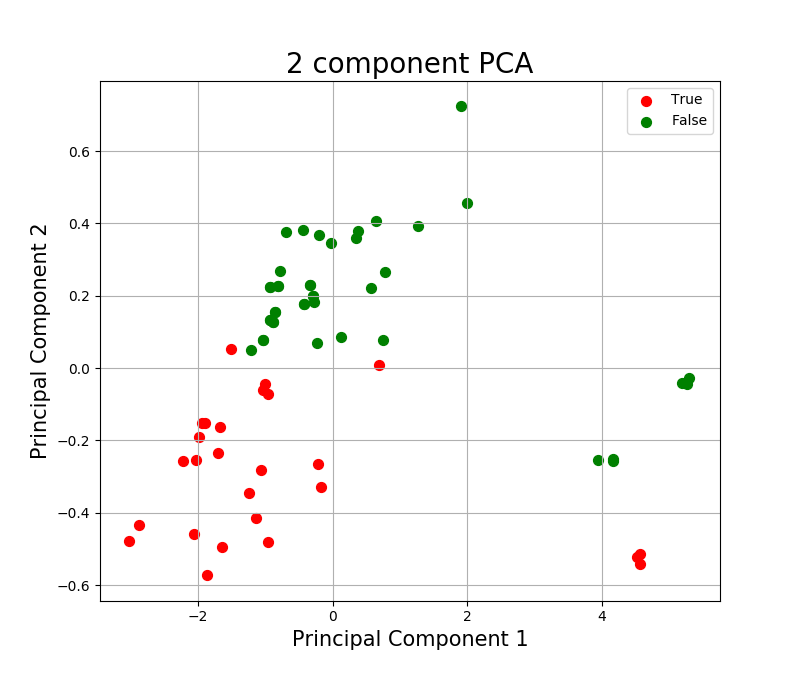
\includegraphics[width=7cm]{pca}
\caption{Plot das Principais Componentes do espectro Raman após normalização dos dados. PC1: 96\% significância, PC2: 2\% de significância. True = Amostra Acima de 10\% Metanol, False = Amostra Abaixo de 10\% Metanol}
\label{pca}
\end{figure}

Então, os dados foram submetidos com todas as suas features a várias configurações diferentes de redes neurais multilayer perceptron tentando classificar os dados como amostra com teor de metanol acima de 10\% ou amostra com teor de metanol inferior a 10\%. Para avaliar a eficácia da rede, avaliou-se o parâmetro chamado Loss, que descreve a evolução do erro a cada iteração da rede neural. O erro deve aproximar-se de zero ao fim das iterações, o que representaria uma assertividade elevada.

Mas, nas configurações utilizadas, a rede neural não apresentou bons resultados como o esperado. O valor do parâmetro Loss estagnou com poucas iterações e ficou muito distante de zero. Por isso, ao realizar os testes a classificação foi sempre a mesma.

Rede Neural com 2 camadas escondidas de 4 e 2 neurônios, figuras \ref{rna_4_2} e \ref{rna_4_2_loss}.

\begin{figure}[ht]
\centering
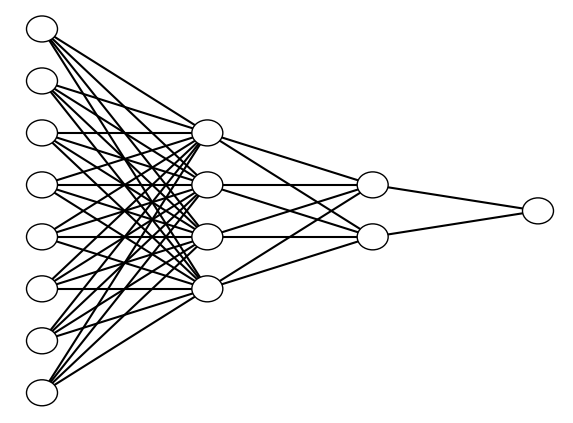
\includegraphics[width=7cm]{rna_4_2}
\caption{Representação da Rede Neural 1024 inputs(foram desenhados apenas 8 inputs para facilitar visualização), com 2 camadas escondidas de 4 e 2 neurônios, respectivamente.}
\label{rna_4_2}
\end{figure}

\begin{figure}[ht]
\centering
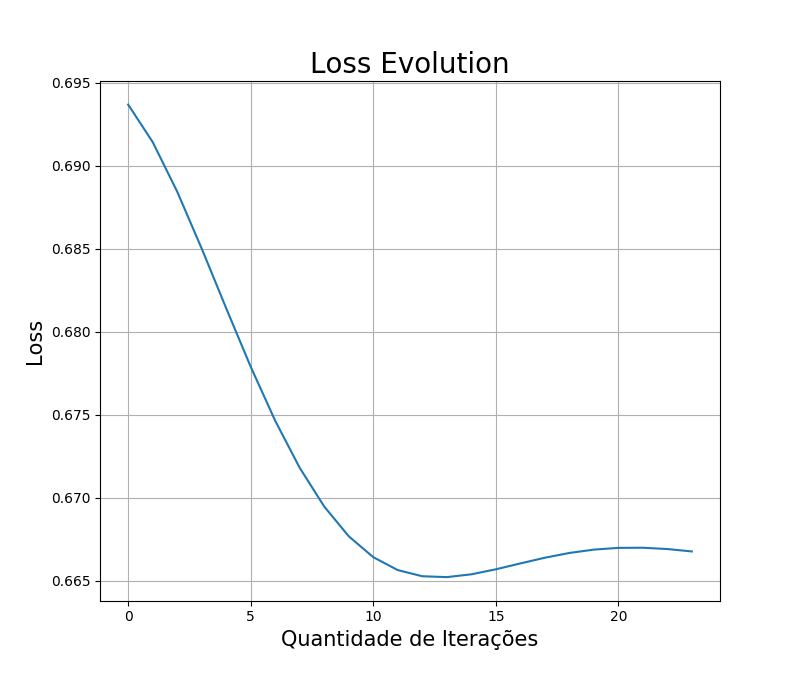
\includegraphics[width=7cm]{rna_4_2_loss}
\caption{Decréscimo do erro a cada iteração da rede neural artificial para a configuração com 2 camadas escondidas de 4 e 2 neurônios, respectivamente}
\label{rna_4_2_loss}
\end{figure}

\vspace{4cm}
Rede Neural com 3 camadas escondidas de 6, 4 e 2 neurônios, figuras \ref{rna_6_4_2} e \ref{rna_6_4_2_loss}.

\begin{figure}[ht]
\centering
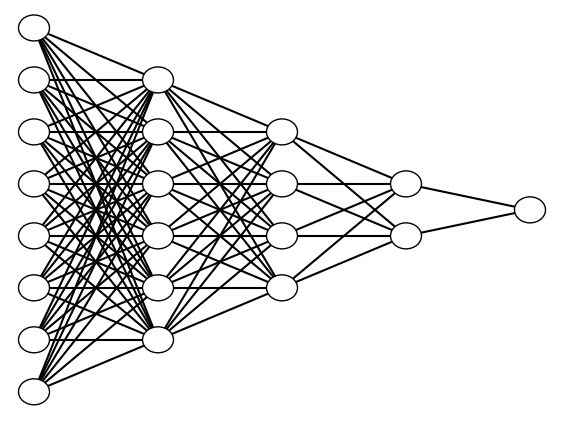
\includegraphics[width=7cm]{rna_6_4_2}
\caption{Representação da Rede Neural 1024 inputs(foram desenhados apenas 8 inputs para facilitar visualização), com 3 camadas escondidas de 6, 4 e 2 neurônios, respectivamente.}
\label{rna_6_4_2}
\end{figure}

\begin{figure}[ht]
\centering
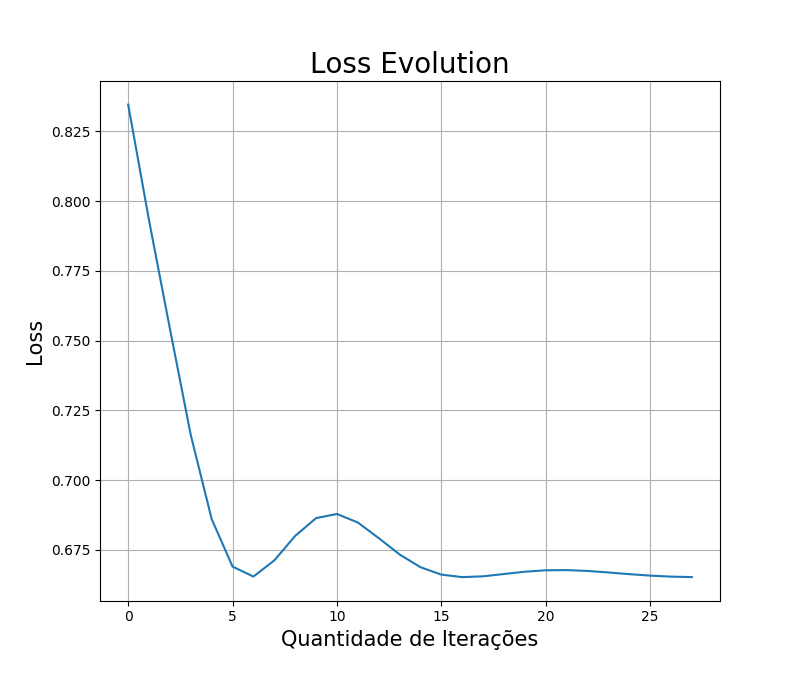
\includegraphics[width=7cm]{rna_6_4_2_loss}
\caption{Decréscimo do erro a cada iteração da rede neural artificial para a configuração com 3 camadas escondidas de 6, 4 e 2 neurônios, respectivamente}
\label{rna_6_4_2_loss}
\end{figure}

\vspace{8cm}
Rede Neural com 3 camadas escondidas de 10, 8 e 6 neurônios, figuras \ref{rna_10_8_6} e \ref{rna_10_8_6_loss}.

\begin{figure}[ht]
\centering
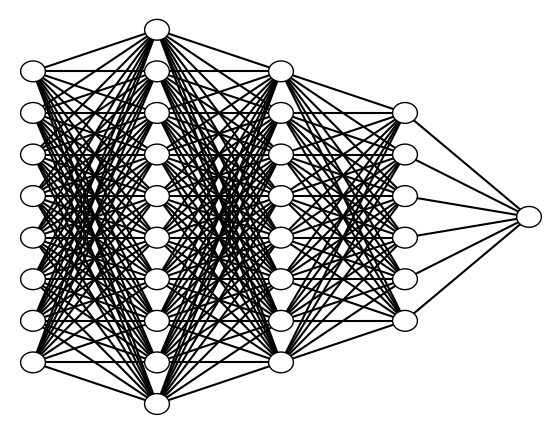
\includegraphics[width=7cm]{rna_10_8_6}
\caption{Representação da Rede Neural 1024 inputs(foram desenhados apenas 8 inputs para facilitar visualização), com 3 camadas escondidas de 10, 8 e 6 neurônios, respectivamente.}
\label{rna_10_8_6}
\end{figure}

\begin{figure}[ht]
\centering
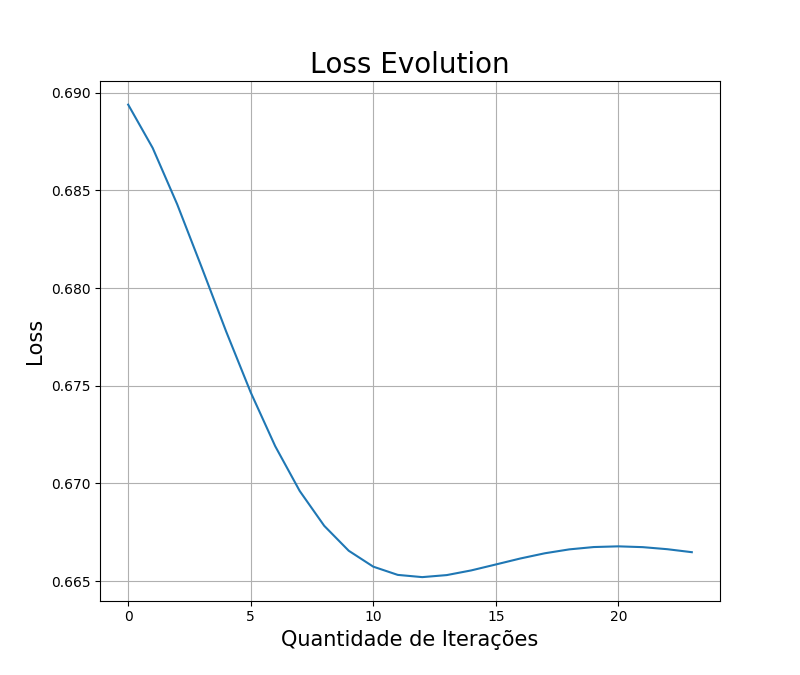
\includegraphics[width=7cm]{rna_10_8_6_loss}
\caption{Decréscimo do erro a cada iteração da rede neural artificial para a configuração com 3 camadas escondidas de 6, 4 e 2 neurônios, respectivamente}
\label{rna_10_8_6_loss}
\end{figure}

Em uma segunda abordagem do problema, a rede neural foi treinada com as duas principais componentes obtidas através do PCA. Para os testes a mesma transformação no espaço realizada nos dados de treinamento foi efetuada nos dados de teste e então estes valores foram aplicados a rede neural. Para está abordagem a rede neural obteve bons resultados, chegando a uma assertividade de 80\% utilizando apenas 1 camadas escondida com 1 neurônio. Na figura \ref{rna_pca_1_loss} pode ser verificado que o loss demora muito mais iterações para estagnar e chega a um valor muito mais próximo de zero que nas abordagens anteriores.

\begin{figure}[ht]
\centering
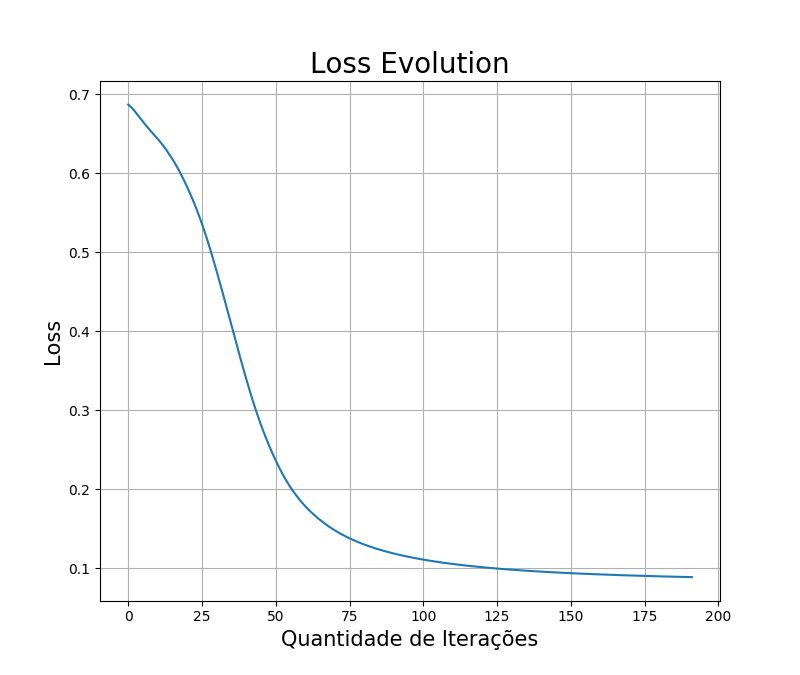
\includegraphics[width=7cm]{rna_pca_1_loss}
\caption{Decréscimo do erro a cada iteração da rede neural artificial para a configuração com 1 camada escondida de 1 neurônio}
\label{rna_pca_1_loss}
\end{figure}

\vspace{4cm}
Foram testadas ainda outras configurações para esta abordagem, contudo a taxa de assertividade cai. Por exemplo, uma rede neural com 3 camadas, de 4, 2, 1 neurônios, respectivamente, teve um taxa de assertividade de 75\%. O que pode ser avaliado como uma situação de overfitting. Na figura \ref{rna_pca_4_2_1_loss} pode ser verificado que a evolução do loss é muito próxima a configuração com 1 camada escondida de 1 neurônio, contudo o erro não chega tão próximo a zero.

\begin{figure}[ht]
\centering
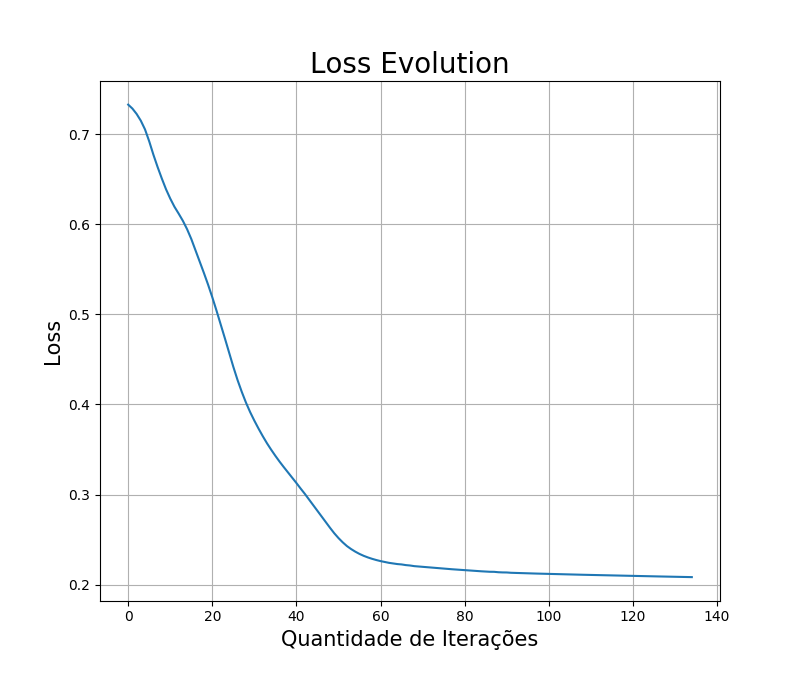
\includegraphics[width=7cm]{rna_pca_4_2_1_loss}
\caption{Decréscimo do erro a cada iteração da rede neural artificial para a configuração com 3 camadas escondida de 4,2,1 neurônios, respectivamente}
\label{rna_pca_4_2_1_loss}
\end{figure}

\vspace{4cm}
\section{Conclusões}
\vspace{1cm} Através da comparação proposta neste trabalho é possivel verificar que em um cenário que a rede neural artificial terá muitas features e poucas amostras para treinamento, é provável que não consiga atingir o resultado esperado.

Contudo ao associar técnicas diferentes, PCA e Redes Neurais Artificiais, os resultados foram assertivos, o que pode evidenciar a capacidade do PCA de extrair as informações relevantes das amostras utilizadas.

Avalia-se também, em que espectros Raman mais complexos, é possível que a variância das componentes da PCA estejam mais difusas. Contudo, uma rede neural, poderia ser treinada não somente com as 2 principais componentes, mas com quantas fossem necessárias para representar uma significância considerável.

Por fim, conclui-se também que o tratamento correto do dados de entrada de uma rede neural pode ser o que irá determinar a assertividade da mesma.
\vspace{2cm}
\section*{Referências}
\vspace{1cm} [1] R. E. De Góes, L. V. M. Fabris, M. Muller, and J. L. Fabris, “Light-
assisted detection of methanol in contaminated spirits,” Journal of
Lightwave Technology, vol. 34, no. 19, pp. 4499–4505, 2016.

\end{document}